%%%%%%%%%%%%%%%%%%%%%%%%%%%%%%
%%%%%%%%%%%%%%%%%%%%%%%%%%%%%
%%%ABSTRA
%   Reduce the margin of the summary:
\def\changemargin#1#2{\list{}{\rightmargin#2\leftmargin#1}\item[]}
\let\endchangemargin=\endlist 


\newcommand\summaryname{Abstract}
\newenvironment{Abstract}%
    {\small\begin{center}%
    \bfseries{\summaryname} \end{center}}

\begin{Abstract}
\begin{changemargin}{1cm}{1cm}
  The aim of this work is to explore the "double descent phenomenon" in artificial neural networks. In addition to the influence of parameters and architecture of the Models, particular emphasis was placed on investigating the second descent of the curve. These investigations should provide insights into the difference between strongly overparameterized and weakly overparameterized neural networks with respect to learned functions and learning process. It is empirically shown that large models can approximate functions that are to be learned from a set of data in a much "simpler" and "smoother" way. The observations should shed light on why such good generalization can be achieved for models with extremely large numbers of parameters. 
\end{changemargin}
\end{Abstract}

%%%%%%%%%%%%%%%%%%%%%%%%%%%%%%
%%%%%%%%%%%%%%%%%%%%%%%%%%%%%
%%%ABSTRACT%%%%%%%%%%%%%%%%%%%%%%



\chapter{Introduction}

One intersection of computer science and mathematics is the field of machine learning. This is an area that has shaped our society and research in recent years and will continue to do so in the future. The role of artificial neural networks is becoming increasingly important in today's world. Without the existence of neural networks, our everyday life would look very different. Although their invention dates back to the 1950s \cite{wikipedia_Machine_learning}, widespread use in many fields of application came only with the 2010s \cite{wikipedia_Machine_learning}. This was partly due to the fact that the computing power of CPUs and GPUs has increased immensely. That's why in today's world the training of larger and larger networks is possible. The current (2022) largest network GPT-3 has 175 billion trainable parameters \cite{romero_2021_tw_ds}. So it is possible even with large training data sets to create a network that learns all inputs by memory. Even though the success of neural networks is immense, the fundamental understanding of this process is not yet completely understood \cite{belkin}. This includes the explanation of the double descent phenomenon, which was described by Belkin in his paper "Reconciling modern machine-learning practice and
the classical bias-variance trade-off". \\
The double descent phenomenon describes the generalization of a model, i.e. its performance on unseen test data, as a function of model size. As the name suggests, the resulting curve contains two phases in which the performance improves monotonically. This means the error rate for unseen data decreases here. With increasing model size the test loss\footnote{a measurement of performance with unseen data} first decreases then increases up to a local maxima, after which a drop in the curve can be observed again. This risk curve can be seen in Figure \ref{double_descent_risk_curve}. Although Belkin's paper published in 2019 has spurred a wave of research, the phenomenon was mentioned as early as 1989 in the paper " Linear and nonlinear extension of the pseudoinverse solution for learning boolean functions" \cite{Vallet_1989}.
In \cite{prehistory_double_descent}, also other papers are described and linked, which have made this discovery, although not directly titled. But the reason why Belkin's paper was cited so often (as of April 20 2022, there were 827 according to google scholar) is probably due to the importance of the topic in today's world. It is becoming easier and easier to build larger networks. In addition, the phenomenon seems like a contradiction to conventional statistical theories of model performance like the bias-variance-trade-off\footnote{a statistical method of analyzing a learning algorithm's expected performance}. This states that training data should not be completely memorized in order to better deal with new unseen data. This is especially important whenever the data set contains a lot of noise. 

\begin{figure}[!htp]
\centering
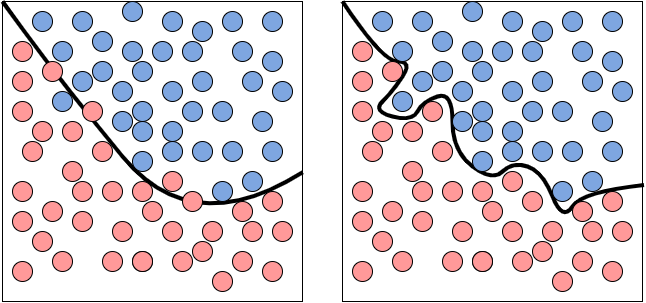
\includegraphics[width= 0.8\linewidth]{Abschlussarbeit_2021/LaTeX/images/tradoff.drawio.png}
\caption{Here is a fictitious seperation problem to see. On the left, all training points were intentionally not memorized in order to be more consistent with new data. On the right, all data points were memorized. This is typical overfitting and can lead to inconsistency with new unseen data.}
\end{figure}

However networks with extremely high capacities interpolate all training data. So they do extreme overfitting i.e. a over adjustment based on the given data, yet their performance is surprisingly good, sometimes even better than models that learn without overfitting. This almost seemingly paradoxical phenomenon is to be investigated in this thesis. For this purpose, the double descent risk curve just described is to be analyzed in detail and assumptions for the cause of the behavior are to be made. 


\begin{figure}[!htp]
\centering
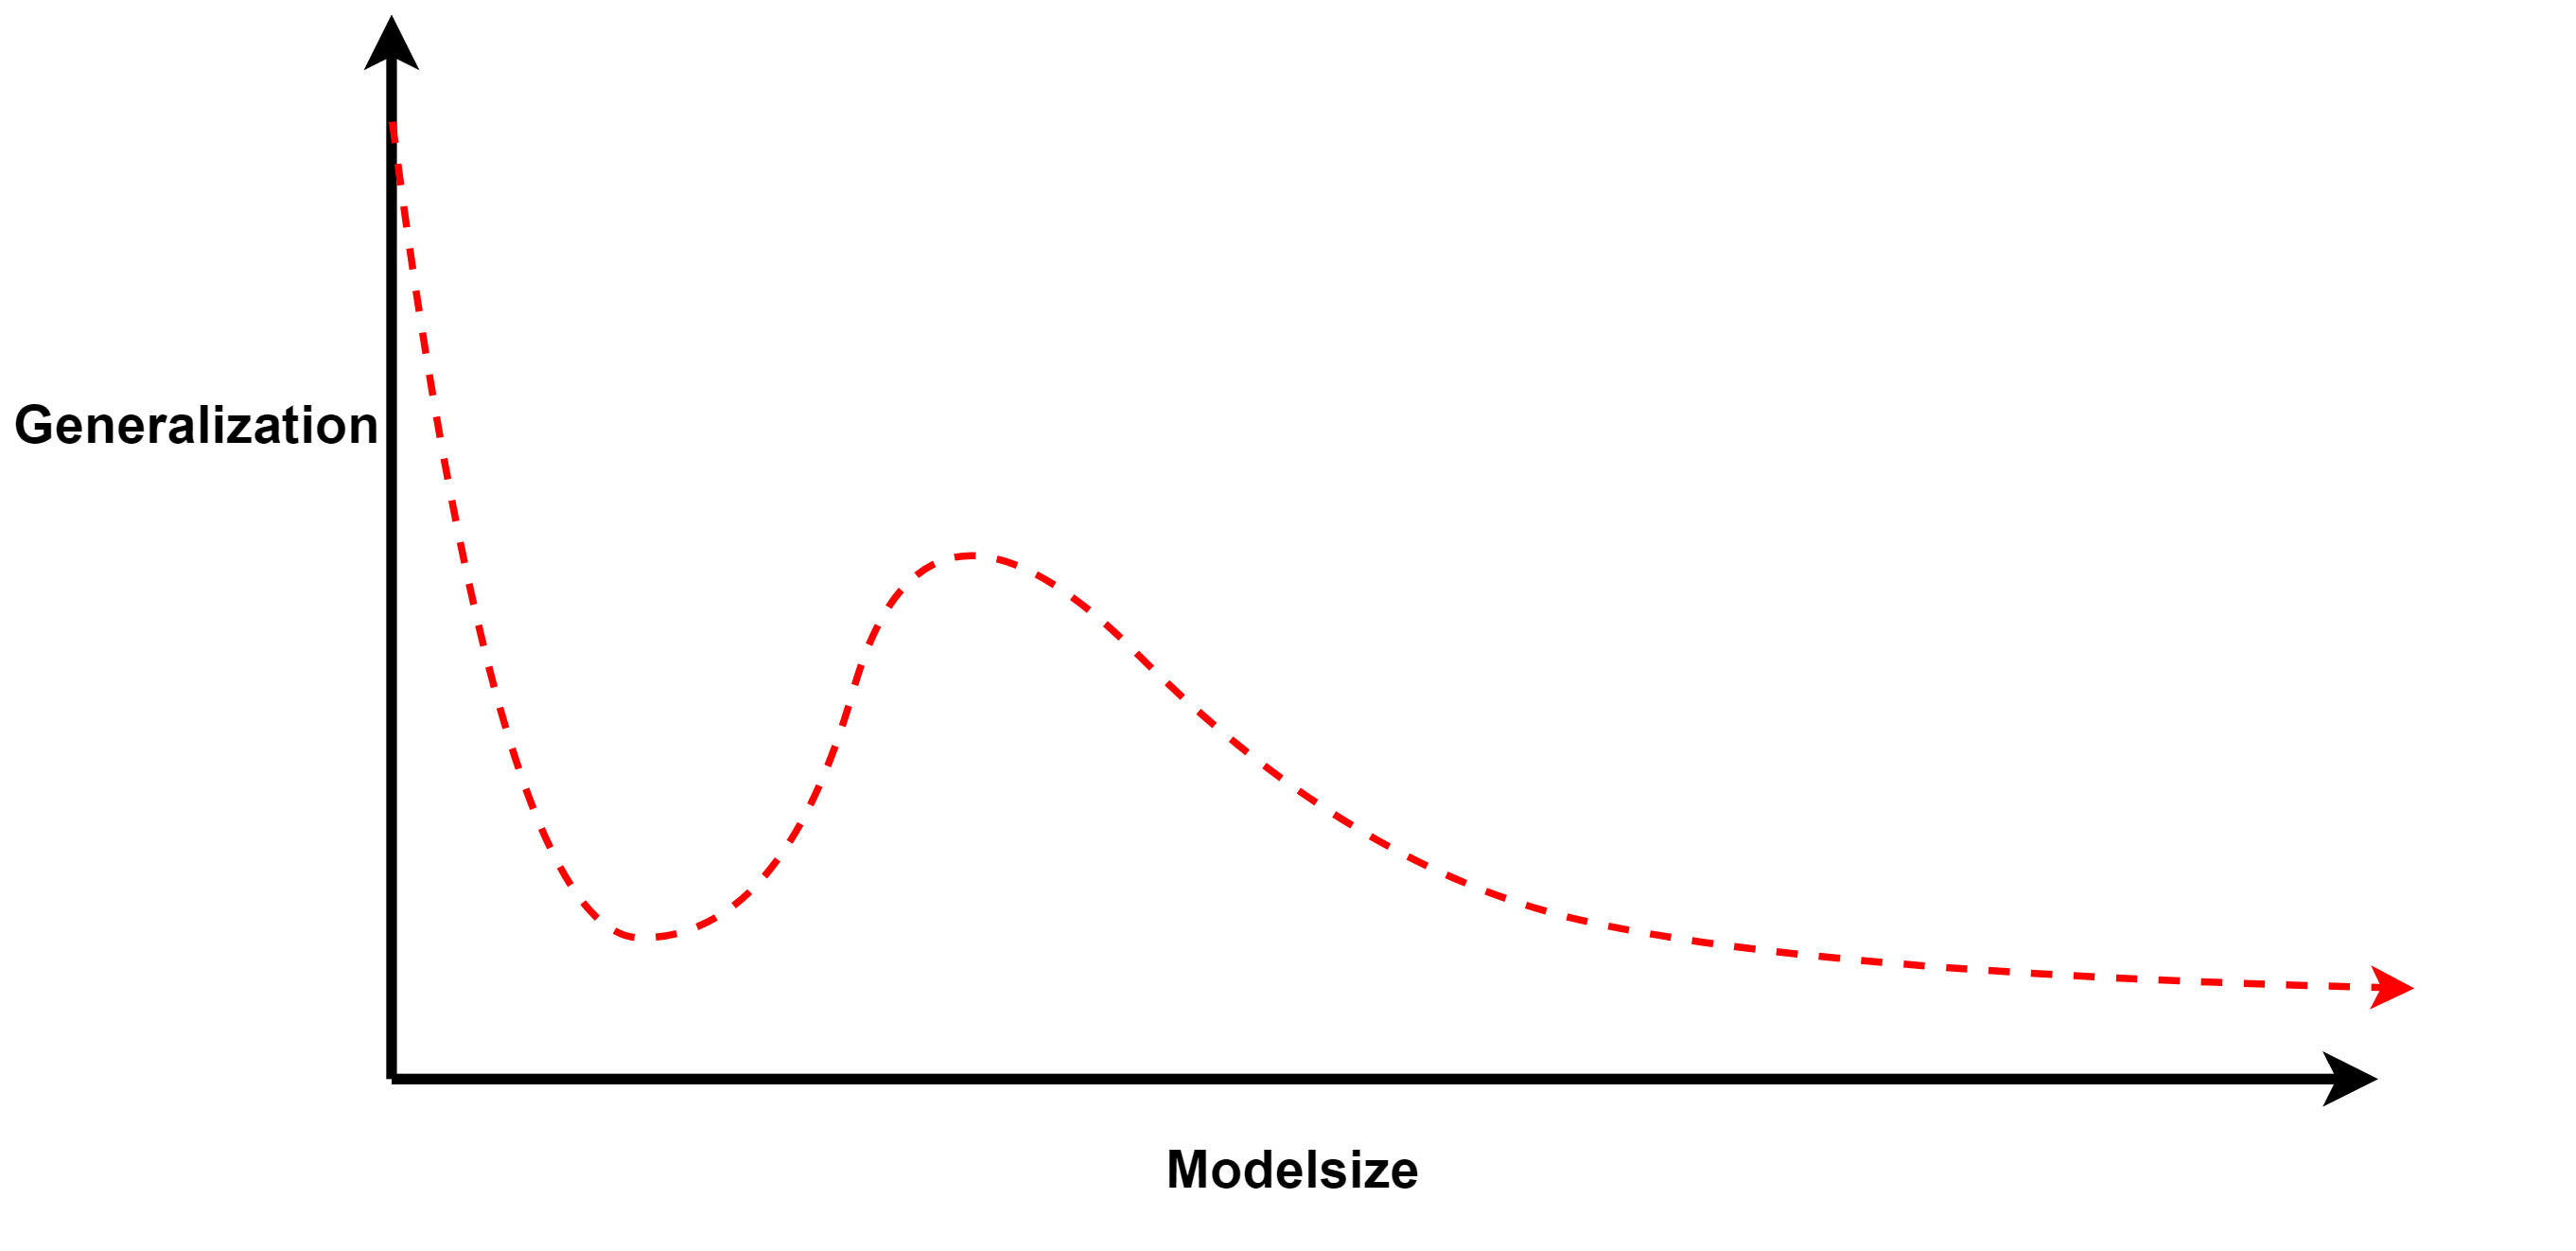
\includegraphics[width= 1\linewidth]{Abschlussarbeit_2021/LaTeX/images/DoubleDescentSkizze.PNG}
\caption{Double descent curve}
\label{double_descent_risk_curve}
\end{figure}

\section{Objective of the Work}

The Thesis is divided into 3 parts. In the first part in chapter 2, the already described Double Descent phenomenon shall be examined more closely. This part is also referred to in the experimental part of the thesis. First the existence of the phenomenon shall be proven and then investigations shall be made, which examine the influence of different parameters on the double descent curve. \\
In chapter 3, the next major part of the thesis, the cause of double descent will be investigated. Particular emphasis will be placed on the possible reasons for the second decrease of the curve. Experiments shall be done, which give information about the changed behavior of larger and larger neural networks. In a detailed analysis possible reasons for the phenomenon will be discussed. \\
The last major part of the work will address the topic of network training, taking into account the phenomenon. Here, among other things, paradoxical effects, which can happen during training, are to be shown. \\
Overall, then, the work focuses on the following questions: Can the shape of the double descent curve be predicted? What influences do certain parameters have on it? What causes the peak of the curve before the second descent? And last but not least the most important question for this thesis: How can the decline of the curve after the peak be explained?




\section{Terms and Definitions}
The following terms are used in the thesis without explanation. 

\begin{itemize}
    \item{\textbf{train loss:}}
    Let $f$ be a learned function of a network and $D = (X_{train},Y_{train})$ be the labeled training data. Thus, the training loss represents a distance between the learned labels and the actual labels using a loss function $l(x,y)$. Thus, the train loss is $l(f(X_{train}),Y_{train})$. If this is zero, then all data points were memorized.
    
    \item{\textbf{test loss:}}
    Same functionality  as the train loss above only that the data points $D = (X_{test},Y_{test})$ are unseen points. Thus, the train loss is $l(f(X_{test}),Y_{test})$.
    
    \item{\textbf{generalization:}}
    Generalization refers to the trained networks ability to adapt properly to new, previously unseen data , drawn from the same distribution as the one used to create the model
    
    \item{\textbf{overfitting:}}
    An over adjustment based on the given data. Focusing too much on training data can lead to poor generalization.
    
    \item{\textbf{underfitting:}}
    An under adjustment based on the given data.
    
    \item{\textbf{test risk:}}
    Also often referred to as empirical risk, describes the risk in predicting unseen data. This risk must be minimized. This is equivalent to minimizing the test loss.
    
    \item{\textbf{SGD:}}
    Stochastic gradient descent (SGD) is an iterative method for optimizing an function. This is achieved by finding minimas in the loss function. Stochasticity is present in it, since the optimization steps are based on random samples only.
    
    \item{\textbf{noise:}}
    Deviation of the data from the actual nominal value. This can happen due to measurement errors or inaccuracies. 
\end{itemize}






